\section{Efeitos de Envelhecimento}
Os efeitos que causam envelhecimentos em circuitos podem ser divididos em dois grupos, os que causam falhas abruptas e os que causam deriva de parâmetros ao longo do tempo. Os principais exemplos do primeiro grupo são os TDDB (time-dependent dielectric breakdown) e EM (electromigration). Já, para o segundo grupo, se tem o NBTI (negative bias temperature instability) e o HCI (hot carrier injection).

Os efeitos do primeiro grupo devem ser tratados estocasticamente, já os do segundo grupo podem ser tratados deterministicamente.

Este trabalho tem como foco os efeitos de envelhecimento de longo prazo, portanto não será tratado sobre os efeitos que causam falhas abruptas.

\subsection{Bias-Temperature Instability}
A variação da tensão de threshold ($\Delta$Vth) dos transistores tipo p e tipo n é a principal característica a ser levada em conta ao analisar o envelhecimento acelerado de tecnologias CMOS. Essa variação acarreta em uma menor velocidade de chaveamento dos transistores.

Uma das principais causas da variação da tensão de threshold é o fenômeno Bias-Temperature Instability (BTI), mais especificamente o Negative BTI (NBTI) afetando os transistores do tipo p e o Positive BTI (PBTI) afetando os transistores do tipo n.

Segundo \cite{Bhardwaj} com dispositivos CMOS de nós tecnológicos cada vez menores, o fenômeno de NBTI se torna um dos principais fatores que determinam a longevidade de transistores PMOS, diferentemente de transistores NMOS, que o principal fator é o HCI (hot-carrier induced degeneration).

Transistores PMOS possuem uma tensão de threshold negativa. O NBTI diminui a tensão de treshold dos transistores PMOS, portanto, aumenta o valor absoluto dela.

\subsubsection{Mecanismos do NBTI}

De acordo com \cite{Zeng} os mecanismos físicos do NBTI podem ser explicados através de três fenômenos não relacionados, que são: a geração de armadilhas de interface, o aprisionamento de lacunas e a geração de armadilhas no óxido do bulk.

O primeiro pode ser explicado pelo modelo de reação-difusão (RD), que diz o NBTI é causado por ligações Si-H quebradas na interface entre o substrato e o oxido do gate. Essas ligações Si-H são formadas na fabricação do dispositivos para impedir que os átomos de silício fiquem com a valência incompleta após a colocação da camada de óxido de silício (SiO\small{2}) sobre o substrato. As ligações pendentes são denominadas estados de interface e podem voltar a ocorrer em condições de estresse.

A Figura \ref{fig:PmosCrossSec} mostra as ligações Si-H na interface entre o gate e o substrato de um transistor PMOS.

\begin{figure}[H]
    \centering
    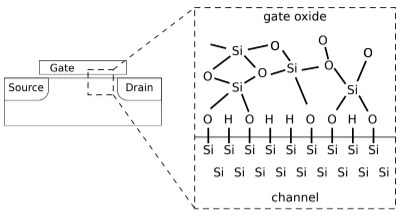
\includegraphics[scale=1]{figures/ReferencialTeorico/Cross section of a PMOS transistor.png}
    \caption{Seção da interface gate-substrato de um transistor PMOS. Fonte: \cite{Lorenz}}
    \label{fig:PmosCrossSec}
\end{figure}

Os estados de interface resultante deterioram parâmetros do transistor. Isso pode ser modelado pelo sistema RD, composto de dois processos: uma reação local e uma difusão dos produtos da reação.

A taxa de geração dessas interfaces é dada pela Equação \ref{eq:TaxaInteface}.

\begin{equation}
    \label{eq:TaxaInteface}
    \diff{N{\textsubscript it}}{t} = K{\scriptstyle F}(N{\scriptstyle 0} - N{\scriptstyle it}) - K{\scriptstyle R}N{\scriptstyle H}(0)N{\scriptstyle it}
\end{equation}

O primeiro termo do lado direito da equação mostra a componente de geração dos estados de interface, já o segundo termo descreve a regeneração das ligações, também denominada annealing reverso, uma característica especial do NBTI.

N\textsubscript{0} representa a quantidade inicial de ligações Si-H, N\textsubscript{it} representa o número de estados de interface e K\textsubscript{R} é a taxa constante de criação de ligações quebradas. No termo de recuperação N\textsubscript{H}(0) representa o número de átomos de hidrogênio na interface do silício com o óxido, K\textsubscript{R} é a taxa constante de annealing reverso das ligações incompletas e átomos de hidrogênio em ligações Si-H.

O lado direito da equação mostra que os estados de interface voltam a diminuir quando a condição de estresse é removida.

A criação de estados de interface é limitado pela difusão dos átomos de hidrogênio, como mostrado na Equação \ref{eq:TaxaDifusao}.

\begin{equation}
    \label{eq:TaxaDifusao}
    \diff{N{\textsubscript it}}{t} = - D{\scriptstyle H}\diff{N{\textsubscript H}}{x} + N{\textsubscript H}\mu{\textsubscript H}E{\scriptstyle ox}
\end{equation}

Onde D\textsubscript{H} representa o coeficiente de difusão, $\mu$\textsubscript{H} representa a mobilidade dos átomos de hidrogênio e E\textsubscript{ox} representa o campo elétrico que atravessa o óxido.

O segundo termo pode ser negligenciado para átomos ou moléculas eletricamente neutros. K\textsubscript{F}, K\textsubscript{R} e D\textsubscript{H} dependem da temperatura. K\textsubscript{F} também depende do campo elétrico aplicado. Isso demonstra que as interfaces só são geradas quando um campo elétrico é aplicado, o que não é necessário para o annealing e para a difusão.

As Equações \ref{eq:TaxaInteface} e \ref{eq:TaxaDifusao} formam um sistema que pode ser resolvido caso seja considerado que N\textsubscript{it} é muito menor que N\textsubscript{0}. A Equação \ref{eq:ResultanteRD} mostra a solução desse sistema e a dependência da quantidade de interfaces com relação o tempo.

\begin{equation}
    \label{eq:ResultanteRD}
    N{\textsubscript {it}} = \sqrt{\frac{K{\scriptstyle F}N{\scriptstyle 0}}{2K{\scriptstyle R}}}(D{\scriptstyle H}t)^{n}
\end{equation}

Onde n representa a constante exponencial de difusão e é sempre menor que 1, de forma que a geração das interfaces irá desacelerar com o tempo.

A variação Vth será proporcional ao N\textsubscript{it}, de forma que poderá ser escrito como mostrado na Equação

Porém, esse fenômeno não explica completamente a geração de NBTI. Um segundo mecanismo relacionado é baseado no aprisionamento de lacuna em defeitos no óxido pre-existentes ou provenientes de estresse elétrico \cite{Butzen}. O campo elétrico que gerado no gate quando o PMOS está negativamente polarizado causa o tunelamento de portadoras do canal nas falhas. Esse fenômeno vem sendo cada vez mais relevante na degradação por NBTI, considerendo que falhas no óxido são mais comuns em transistores high-k.

% Transistors with high-κ dielectric have higher density of pre-existing defects. From this point-of-view, hole trapping/detrapping is becoming the dominant contributor to NBTI degradation (KACZER, 2010).

Cada um desses fenômenos contribui para a variação da tensão de treashold resultando na equação \ref{eq:SomaVth}. Onde V\textsubscript{IT} á a contribuição das armadilhas de interface, V\textsubscript{HT} é a contribuição do aprisionamento em defeitos pré existentes e V\textsubscript{OT} é a contribuição do aprisionamento em defeitos gerados eletricamente.

\begin{equation}
    \label{eq:SomaVth}
    \Delta V{\textsubscript {th}} = \Delta V{\textsubscript {IT}} + \Delta V{\textsubscript {HT}} + \Delta V{\textsubscript {OT}}
\end{equation}

A Equação \ref{eq:VthTempo} mostra uma aproximação da variação da tensão de treshold ao longo do tempo considerando um nó tecnológico específico e um certo conjunto de condições ambientais \cite{Butzen}.

\begin{equation}
    \label{eq:VthTempo}
    \Delta Vth = A(TSP.t)^n
\end{equation}

Onde A é uma constante que depende da tecnologia, t é o tempo, n é a constante exponencia do NBTI e TSP é a probabilidade do transistor estar negativamente polarizado.
\subsubsection{Gerando NBTI}
\label{sec:GerandoNbti}
Muitos estudos já foram realizados para determinar em que condições o NBTI ocorre com mais facilidade em circuitos CMOS.

O fenômeno NBTI normalmente ocorre em transistores do tipo p operando com tensão de gate negativa em temperaturas variando de 100ºC a 250ºC \cite{Davidovic}. Os campos elétricos devem ser na faixa dos 6MV/cm, valores encontrados durante o burn-in do componente, porém com transistores cada vez menores, esses campos podem ocorrer durante a operação normal de dispositivos de alta performance \cite{Schroder}. A Figura \ref{fig:CampoEletricoAno} mostra o aumento do campo elétrico que atravessa o óxido em transistores CMOS ao longo dos anos.

\begin{figure}[H]
    \centering
    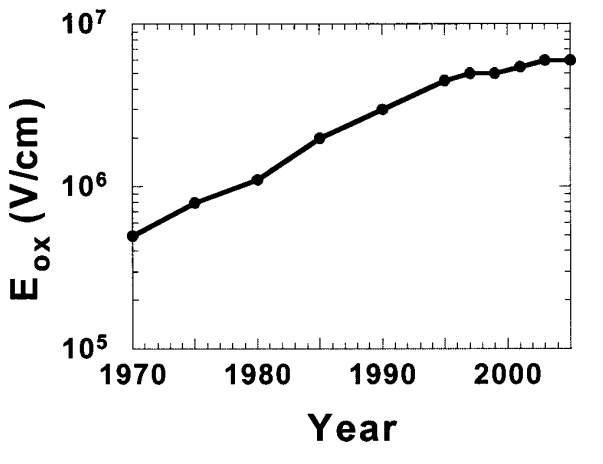
\includegraphics[scale=0.5]{figures/ReferencialTeorico/CampoEletricoAno.png}
    \caption{Campo elétrico no óxido em dispositivos CMOS ao longo dos anos. Fonte: \cite{Schroder}}
    \label{fig:CampoEletricoAno}
\end{figure}

% Typical stress temperatures lie in the 100– 250 °C range with oxide electric fields typically below 6 MV/cm, i.e., fields below those that lead to hot carrier degradation. Such fields and temperatures are typically encountered during burn in, but are also approached in highperformance ICs during routine operation.

Para aplicar o efeito de NBTI no dispositivo ensaiado no trabalho \cite{Davidovic}, os pesquisadores o estressaram por 2000 horas, aplicando tensões negativas de 30 a 45V no gate (com fonte e dreno aterrados) em uma temperatura de variando de 125 a 175ºC.

O trabalho de \cite{Bhardwaj} desenvolveu um modelo preditivo para NBTI em dispositivos CMOS de nó tecnológico de 45nm, que alcançou estimativas precisas da degradação em longo prazo da tensão de threshold de transistores PMOS devido ao fenômeno.

Um outro trabalho \cite{Grossi}, realizou simulações para analisar os efeitos do BTI em amplificadores operacionais, e viu que o ganho DC, a frequência de corte e o slew rate são significativamente degradados em AMPOPs operando em malha aberta. Já para Ampops operando com realimentação negativa apenas a frequência de corte mostrou uma degradação significativa.

Alguns trabalhos, inclusive, realizaram estudos dos efeitos de NBTI em osciladores em anel. Um deles \cite{Lorenz} mostra uma degradação de 5\% com 144 horas de exposição à 125°C. Já outro \cite{Sato}, que estudou métodos para diminuir o efeito de NBTI em osciladores em anel, resultou uma degradação de 0,25\%, com 42 horas de exposição, porém à apenas 85°C. Um terceiro trabalho \cite{Linder} propõe topologias de osciladores em anel que permitem estudar em separado os efeitos do PBTI, nele foi medida um degradação de 1,8\% considerando apenas o PBTI, 2,2\% considerando apenas o NBTI e 3,9\%  considerando apenas os dois efeitos combinados tendo sido realizado um estresse de 2 horas e 47 minutos (10000 segundos) segundos à 125°C.

